
%----------------------------------------------------------------------------------------
%	PREAMBUŁA
%----------------------------------------------------------------------------------------


\documentclass[12pt]{article}
\usepackage[polish]{babel}
\usepackage{polski}
\usepackage[utf8]{inputenc}
\usepackage{graphicx}
\usepackage{fancyhdr}
\usepackage{float}
\usepackage{graphicx}
\usepackage[hidelinks]{hyperref}
\usepackage{verbatim}
\usepackage{amsmath}
\usepackage{rotating}
\usepackage{listings}
\usepackage{xcolor}
\usepackage{subcaption}

\definecolor{lgray}{gray}{0.96}
\definecolor{lbcolor}{rgb}{0.9,0.9,0.9}
\lstset{
    framesep=2pt,
    breaklines=true,
    breakatwhitespace=true,
    basicstyle=\footnotesize,
    aboveskip={0.75\baselineskip},
    columns=flexible,
    showstringspaces=false,
    breaklines=true,
    prebreak = \raisebox{0ex}[0ex][0ex]{\ensuremath{\hookleftarrow}},
    frame=single,
    rulecolor=\color{lgray},
    showtabs=false,
    showspaces=false,
    showstringspaces=false,
    backgroundcolor=\color{lgray},
    identifierstyle=\ttfamily,
    keywordstyle=\color[rgb]{0,0,1},
    commentstyle=\color[rgb]{0.0,0.26,0.15},
    stringstyle=\color[rgb]{0.627,0.126,0.941}
}

\graphicspath{{static/}} 

\title{Dokumentacja projektu}
\author{Aleksandra Poręba}

\makeatletter
\let\thetitle\@title
\let\theauthor\@author
\let\thedate\@date
\makeatother

%----------------------------------------------------------------------------------------
%	STRONA TYTUŁOWA
%----------------------------------------------------------------------------------------
\begin{document}
\begin{center}
\textsc{\normalsize Wydział Fizyki i Informatyki Stosowanej}\\[2.0cm] 

\includegraphics[scale = 1]{logo.pdf}\\[1cm] 
\textsc{\Large Zaawansowane Technologie Internetowe}\\[0.4cm] 


{ \huge \bfseries \LARGE{Dokumentacja projektu} }\\[0.2cm] 

\flushright \Large Aleksandra Poręba

\vfill 

\center {\today}\\[2cm] 


\pagebreak 

\end{center}

%----------------------------------------------------------------------------------------
%	SPIS TREŚCI
%----------------------------------------------------------------------------------------
\setcounter{tocdepth}{2}
\tableofcontents
\pagebreak

%----------------------------------------------------------------------------------------
%	ZAWARTOŚĆ
%----------------------------------------------------------------------------------------

\pagestyle{fancy}
\fancyhf{}

\rhead{\theauthor}
\lhead{\thetitle}
\cfoot{\thepage}

\section{Wstęp}
Niniejszy dokument stanowi dokumentację projektu zrealizowanego w ramach przedmiotu \textit{Zaawansowanie Technologie Internetowe}. Została przygotowana aplikacja 
z wykorzystaniem technologii \textit{Java API for RESTful Web Services}.

Do stworzenia aplikacji klienta został wykorzystany framework \textit{ReactJS} z wykorzystaniem dodatkowych bibliotek i pakietów, takich jak \textit{redux}, \textit{axios}, \textit{moment.js} czy \textit{Materialize}.

Do projektu została również przygotowana baza danych \textit{PostgreSQL} umieszczona w środowisku chmurownym \textit{ElephantSQL}. Zarówno serwer jak i aplikacja klienta zostali umieszczeni w ramach chmury \textit{IBM Cloud}. Są dostępne pod poniższymi adresami:
\begin{itemize}
\item serwer \\ \url{https://alporeba-zti-projekt.eu-gb.mybluemix.net/db/rest/}
\item klient \\ \url{https://alporeba-zti-projekt-client.eu-gb.mybluemix.net/}
\end{itemize}

\pagebreak
\section{Aplikacja serwera}
\subsection{Funkcjonalności}
W ramach projektu został stworzony serwer, którego zadaniem jest odpytywanie bazy danych o odpowiednie informacje. Został on przygotowany z użyciem technologii \textit{JPA} oraz \textit{AspectJ} do logowania działania serwera.

Aby przybliżyć funkcjonalności serwera konieczna jest znajomość organizacji bazy danych, przedstawiona poniżej.

\begin{figure}[H]
\centering
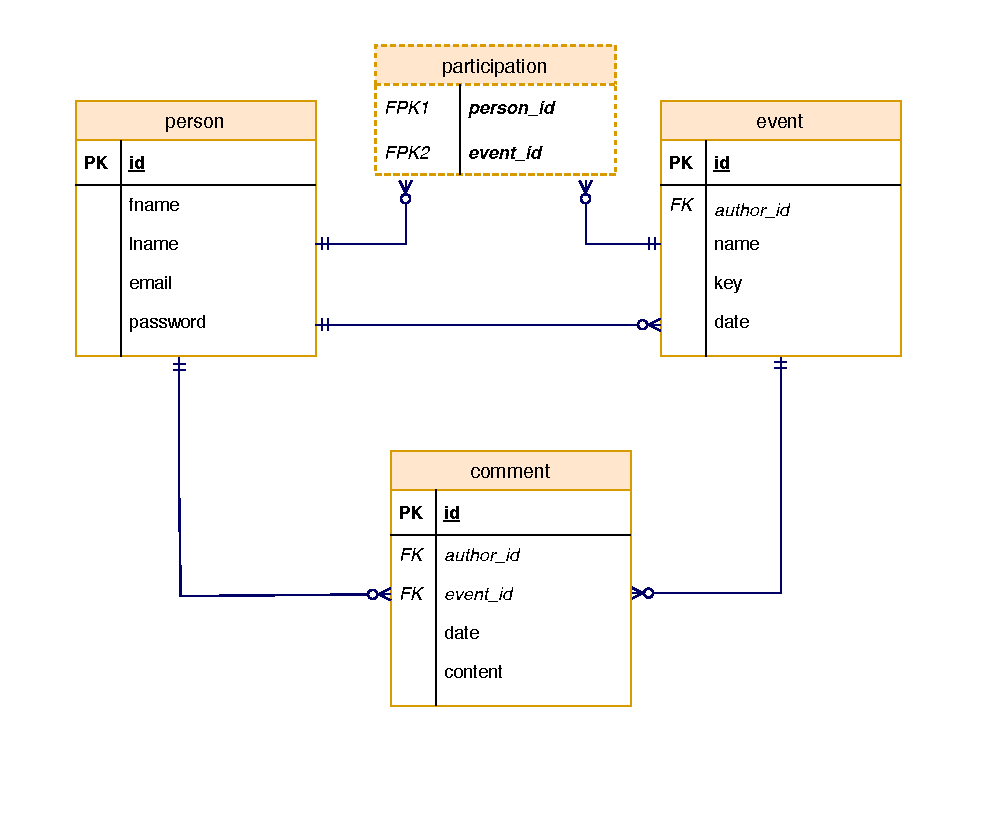
\includegraphics[width=0.8\textwidth]{erd.pdf}
\caption{Diagram ERD bazy danych.}
\end{figure}

Zgodnie z czterema tabelami, funkcjonalności serwisu \textit{RESTful} zostały podzielone na cztery części: 
\begin{itemize}
\item \textit{person} - obsługujące działania związane z użytkownikami, 
\item \textit{event} - obsługujące działania związane z wydarzeniami, 
\item \textit{comment} - komentarze do wydarzeń,
\item \textit{participation} - wzięcie udziału przez użytkownika w wydarzeniu.
\end{itemize}

Do każdej z 4 części możliwe są operacje \textit{CRUD - Create, Read, Update, Delete} dostępne poprzez odpowiednie metody \textit{Http}. Odczytać można zarówno wszystkie rekordy, jak i pojedynczy, identyfikowany przez id. Poniżej znajduje się przykładowe zapytanie i odpowiedź:

\begin{lstlisting}[ mathescape=true, basicstyle=\scriptsize]
https://alporeba-zti-projekt.eu-gb.mybluemix.net/db/rest/person

[[1,"Captain","America","ca@marvel.com","dummypass"],[2,"Iron","Man","im@marvel.com","dummypass"]]
\end{lstlisting}

Zostały przygotowane również zapytania bardziej szczegółowe, na potrzeby aplikacji klienta, na przykład:

\begin{lstlisting}[ mathescape=true, basicstyle=\scriptsize]
https://alporeba-zti-projekt.eu-gb.mybluemix.net/db/rest/comment/event/12

[["Ryby sa fajne","2020-06-29 05:53:27",5,12,1,"America","Captain"]]
\end{lstlisting}

Wszystkie szczegółowe zapytania to:
\begin{itemize}
\item \textit{/person/email/\{email\}} - odczytanie danych osoby, identyfikując ją przez e-mail,
\item \textit{/comment/event/\{id\}} - odczytanie wszystkich komentarzy dla danego wydarzenia,
\item \textit{/event/key/\{key\}} - odczytanie wydarzenia identyfikowanego za pomocą klucza,
\item \textit{/event/details/\{id\}} - odczytanie detali wydarzenia, np również danych organizatora,
\item \textit{/event/author/\{id\}} - odczytanie wszystkich wydarzeń, których dana osoba jest organizatorem,
\item \textit{/event/person/\{id\}} - odczytanie wszystkich wydarzeń, w których dana osoba bierze udział,
\end{itemize}

Wszystkie zapytania można testować za pomocą narzędzia \verb\curl\ dostępnego na maszynach wirtualnych.

\subsection{Budowa}
Na diagramie poniżej została przedstawiona organizacja plików po części serwera. 

\begin{figure}[H]
\centering
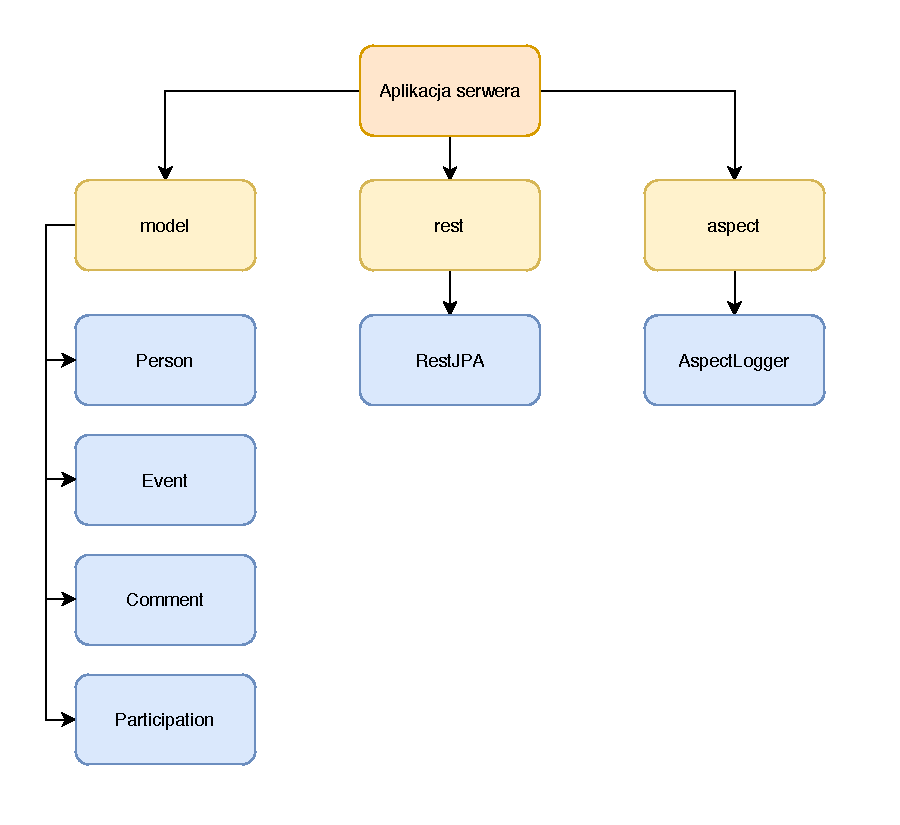
\includegraphics[width=0.9\textwidth]{server.pdf}
\caption{Budowa aplikacji serwera.}
\end{figure}

Przygotowanie zostały 3 pakiety: 
\begin{itemize}
\item \textit{model} zawierający klasy \textit{POJO} odpowiadające tabelom w bazie,
\item \textit{api} obsługujący wysyłanie zapytań,
\item \textit{aspect} zapewniające aspektowe logowanie działania serwera.
\end{itemize}

Poszczególne klasy oraz ich metody zostały szczegółowo w dokumentacji \textit{JavaDoc}.

\pagebreak
\section{Aplikacja klienta}
Do stworzenia aplikacji klienta został wykorzystany framework \textit{React.js}. Udostępnione funkcjonalności, oraz budowa aplikacji zostały przedstawione poniżej. 

\subsection{Funkcjonalności}

Aplikacja klienta udostępnia możliwość zapisywania się na prywatne wydarzenia, znajdowane według klucza. Osoby zapisane mogę dodawać i usuwać komentarze do danego spotkania, a także je opuścić.

Użytkownik ma również możliwość tworzenia nowych wydarzeń, edytowania istniejących, których jest właścicielem, a także usuwanie ich.

Został przygotowany również serwis autoryzacji użytkownika - logowanie się, tworzenie konta, edycja danych.

Instrukcje poszczególnych operacji zostały przedstawione w rozdziale \ref{sec:guide}.

\subsection{Budowa}
Struktura plików aplikacji klienta została podzielona na dwie części: \verb\store\ zawierający pliki potrzebne do zarządzania magazynem danych oraz \verb\components\ zawierający wszystkie komponenty. Schemat organizacji został przedstawiony poniżej.

\begin{figure}[H]
\centering
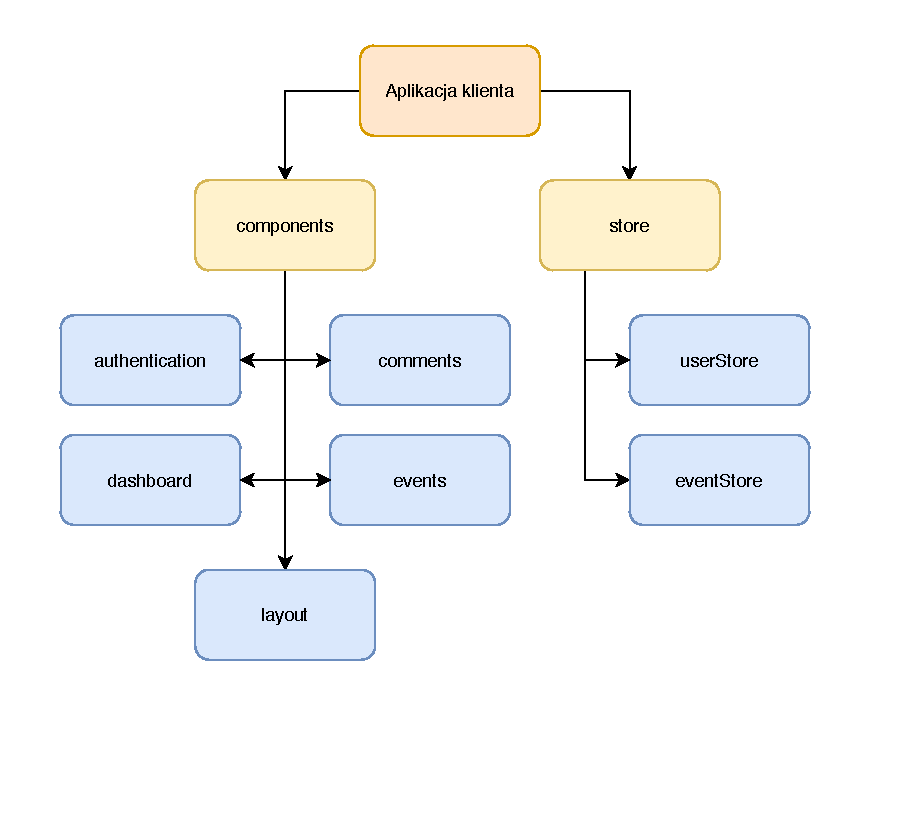
\includegraphics[width=0.9\textwidth]{client.pdf}
\caption{Budowa aplikacji klienta.}
\end{figure}

Komponenty zostały podzielone na pięć kategorii:
\begin{itemize}
\item \textit{authentication} - obsługa uwierzytelnienia - logowanie, zakładanie konta, edycja danych,
\item \textit{comments} - dodawanie, usuwanie oraz wyświetlanie komentarzy,
\item \textit{dashboard} - podstawowe komponenty strony głównej użytkownika oraz managera spotkań,
\item \textit{events} - działanie związane z wydarzeniami, podzielone na dwie części - część do strony głównej - wyświetlanie listy, szczegółów, oraz część do managera spotkań, z możliwością dodawania wydarzeń, edycji, usuwania,
\item \textit{layout} - komponenty związane z wyglądem aplikacji.
\end{itemize}

Do obsługi danych aplikacji została wykorzystana biblioteka \textit{Redux}. Zostały stworzone dwa magazyny, zgodnie z podziałem funkcjonalności aplikacji klienta: 
\begin{itemize}
\item jeden do obsługi zdarzeń: dodawania ich, usuwania, komentarzy, zapisu na wydarzenia,
\item oraz do obsługi użytkownika - logowania, tworzenia i edycji konta, pobierania danych użytkownika.
\end{itemize}

W akcjach wysyłane są zapytania \textit{HTTP} do serwera za pomocą pakietu \textit{axios}. Otrzymane odpowiedzi są odpowiednio parsowane i zapisywane do odpowiednich magazynów. Stamtąd odczytywane są przez komponenty, które uaktualniają odpowiednie widoki.

Kod źródłowy aplikacji klienta został dokumentowany za pomocą adnotacji \textit{JSDoc}.

\pagebreak
\section{Testowanie}

Działanie serwera zostało szczegółowo przetestowane za pomocą testów jednostkowych. Do ich wykonania zostały użyte takie narzędzia jak \textit{curl} oraz przeglądarka \textit{Chromium}. Przykładowe testy zostały przedstawione poniżej.

\pagebreak
\section{Wdrożenie}

\subsection{Serwer}
Aplikację serwera można uruchomić na lokalnym serwerze w środowisku \textit{Ecplise}. Należy wykonać następujące operacje:


Tak uruchomiony serwer jest dostępny pod adresem: \url{TODO}.

Aby wdrożyć aplikację do chmury \textit{IBM Cloud} należy najpierw przygotować plik \textit{manifest.yml}. Przykładowy plik przedstawiono poniżej.
\begin{lstlisting}[ mathescape=true, basicstyle=\scriptsize]
manifest
\end{lstlisting}

Również konieczne jest archiwum \textit{war} proejktu serwera, które możemy stworzyć za pomocą środowiska \textit{Ecplise}. W tym celu należy wybrać kolejno:

Następnie, należy wykonać następujące polecenia:
\begin{lstlisting}[ mathescape=true, basicstyle=\scriptsize]
ibmcloud login
ibmcloud cf target ?
ibmcloud cf push
\end{lstlisting}

\subsection{Klient}
Aplikację klienta można uruchomić zarówno na maszynach wirtualnych używanych w ramach przedmiotu, jak i na własnym, lokalnym komputerze. Warunkiem jest posiadanie narzędzia \verb\npm\.

Przed uruchomieniem należy uzupełnić plik \verb+\meetup-client\ser\config.js+ w którym powinien znaleźć się link do serwera.

Aby uruchomić lokalnie aplikację należy wykonać następujące polecenia:
\begin{lstlisting}[]
cd meetup-client
npm install
npm start
\end{lstlisting}

Aplikacja zostanie uruchomiona lokalnie, najczęściej na porcie \verb\3000\.

Aby wdrożyć aplikację do środowiska \textit{IBM Cloud} należy najpierw przygotować plik \textit{manifest.yml}. Przykładowy plik przedstawiono poniżej.
\begin{lstlisting}[ mathescape=true, basicstyle=\scriptsize]
manifest
\end{lstlisting}

Powinien on znaleźć się w katalogu \verb\meetup-client\. Następnie, aby zbudować aplikację klienta i wdrożyć ją do chmury należy wykonać polecenia:
\begin{lstlisting}[ mathescape=true, basicstyle=\scriptsize]
npm build
...

ibmcloud login
ibmcloud cf target ?
ibmcloud cf push
\end{lstlisting}

\pagebreak
\section{Podręcznik użytkownika}
\label{sec:guide}
Poniższy rozdział zawiera instrukcję użytkownika do obsługi aplikacji klienta.
\subsection{Logowanie oraz tworzenie konta}
Gdy klient uruchomi aplikację, wyświetlony zostanie domyślny ekran.

\begin{figure}[H]
\centering
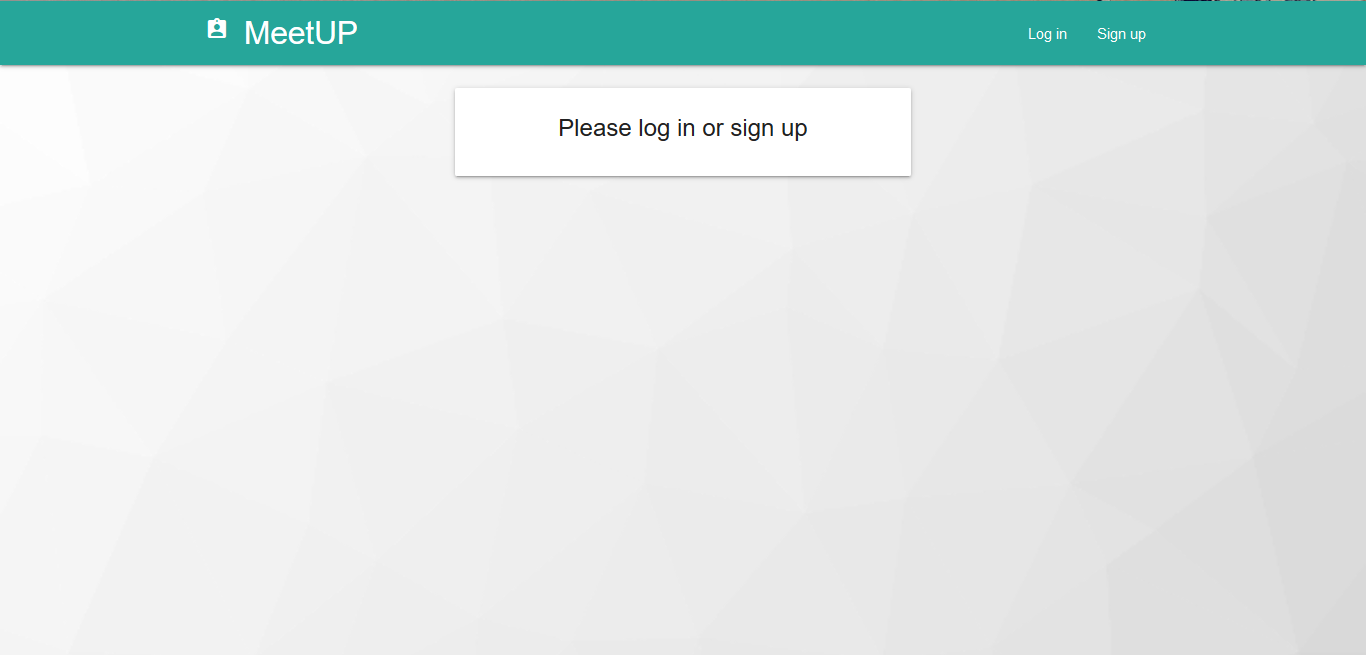
\includegraphics[width=0.9\textwidth]{meetup_main.png}
\caption{Strona główna aplikacji dla użytkownika niezalogowanego.}
\end{figure}

Na górze strony znajduje się pasek nawigacji, za pomocą którego użytkownik może się zalogować lub zarejestrować. Ekrany z poszczególnymi formularzami zostały przedstawione poniżej.

\begin{figure}[H]
\centering
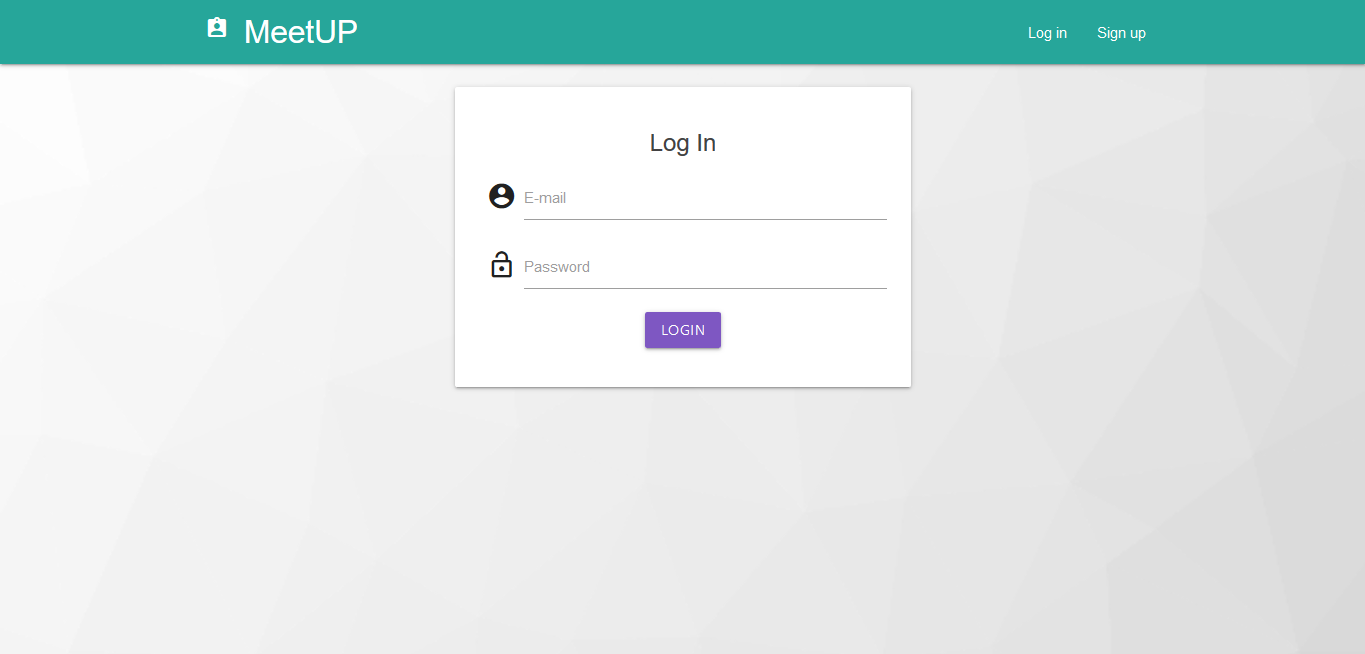
\includegraphics[width=0.9\textwidth]{meetup_login.png}
\caption{Formularz logowania.}
\end{figure}

\begin{figure}[H]
\centering
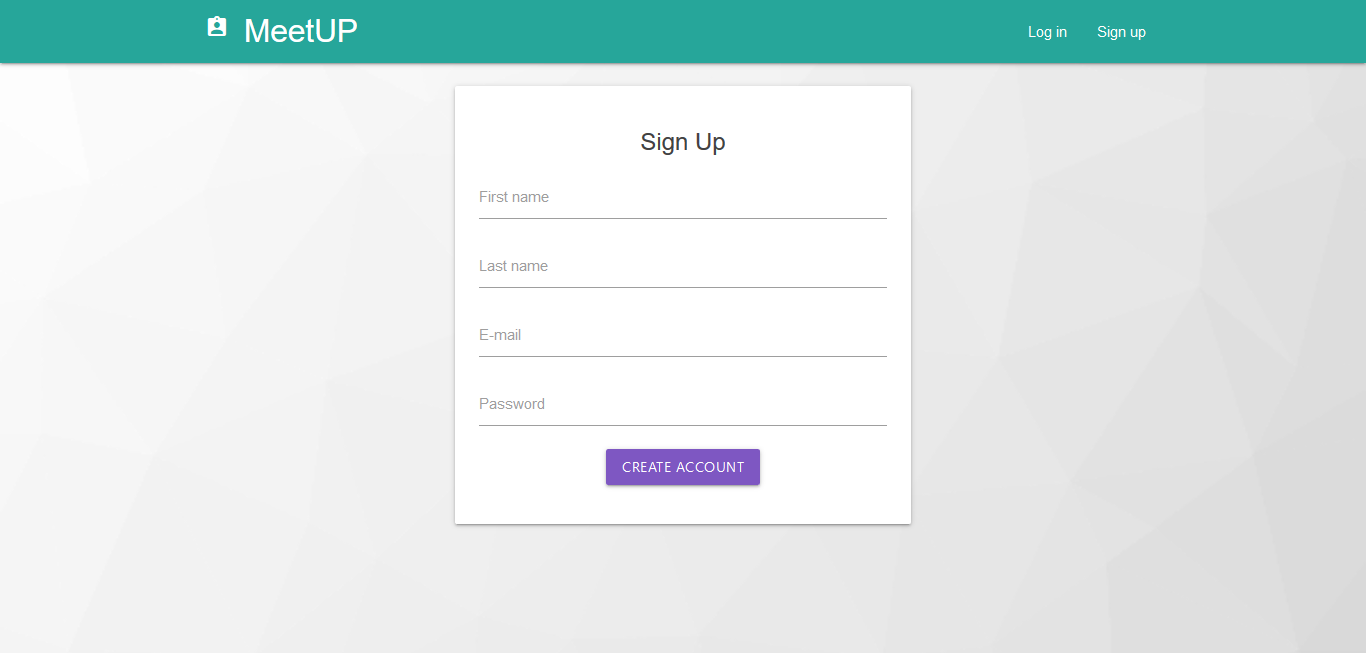
\includegraphics[width=0.9\textwidth]{meetup_signup.png}
\caption{Formularz rejestracji.}
\end{figure}

Gdy użytkownik poda nieprawidłowe dane, na przykład hasło przy rejestracji zostanie wyświetlony odpowiedni komunikat.

\begin{figure}[H]
\centering
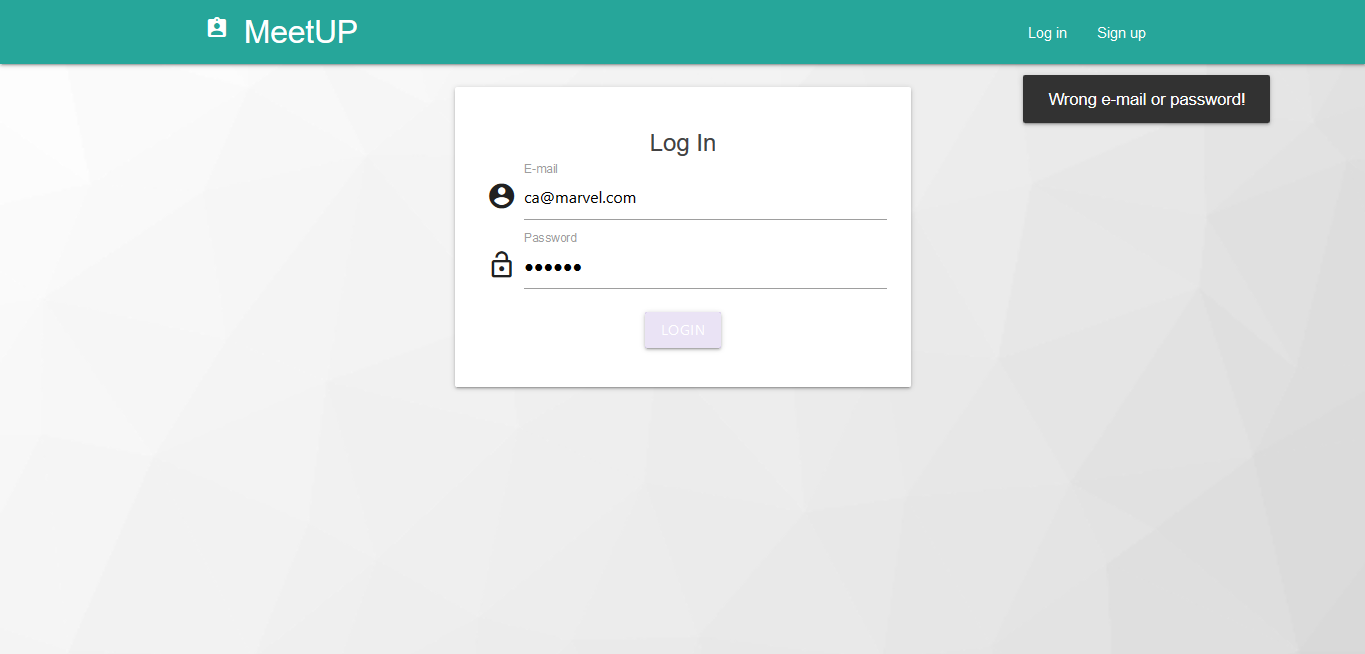
\includegraphics[width=0.9\textwidth]{meetup_login_error.png}
\caption{Formularz błędnego logowania.}
\end{figure}

Gdy logowanie lub rejestracja powiedzie się użytkownikowi ukaże się strona główna aplikacji.

\begin{figure}[H]
\centering
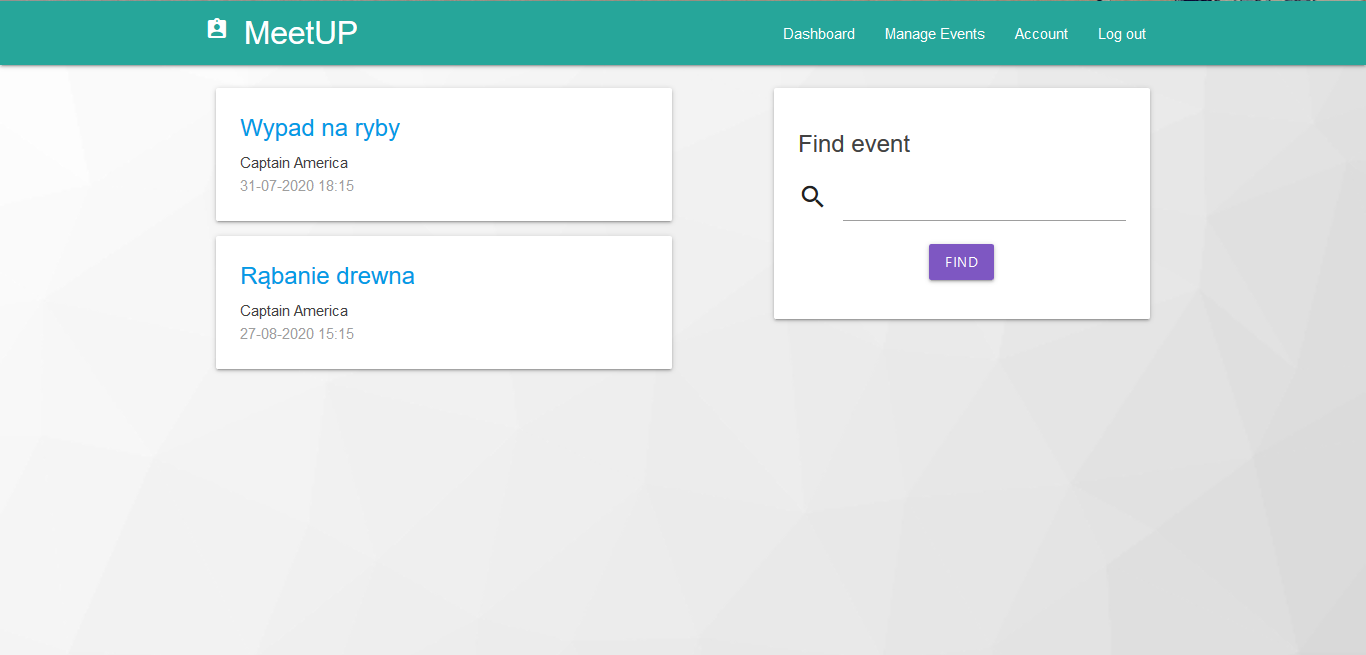
\includegraphics[width=0.9\textwidth]{meetup_dashboard.png}
\caption{Strona główna aplikacji dla użytkownika zalogowanego.}
\end{figure}

Opcje paska nawigacji są już inne, zgodne z uprawnieniami użytkownika zalogowanego. Może on przeglądać wydarzenia, w których bierze udział, zarządzać wydarzeniami, których jest autorem, edytować swoje dane, czy też wylogować się. Operacje te zostaną opisane w dalszej części.

\subsection{Wyszukiwanie wydarzenia i zapis}
Wydarzenia, na które zapisał się użytkownik wyświetlone są po lewej stronie w kolejności chronologicznej. Nie są wyświetlane spotkania, których data już minęła. Po prawej stronie użytkownik może wyszukać nowe wydarzenia, na które może się zapisać. Identyfikacja następuje za pomocą unikalnego klucza, który ustala organizator, aby żadna osoba postronna nie miała dostępu do wydarzenia.

\begin{figure}[H]
\centering
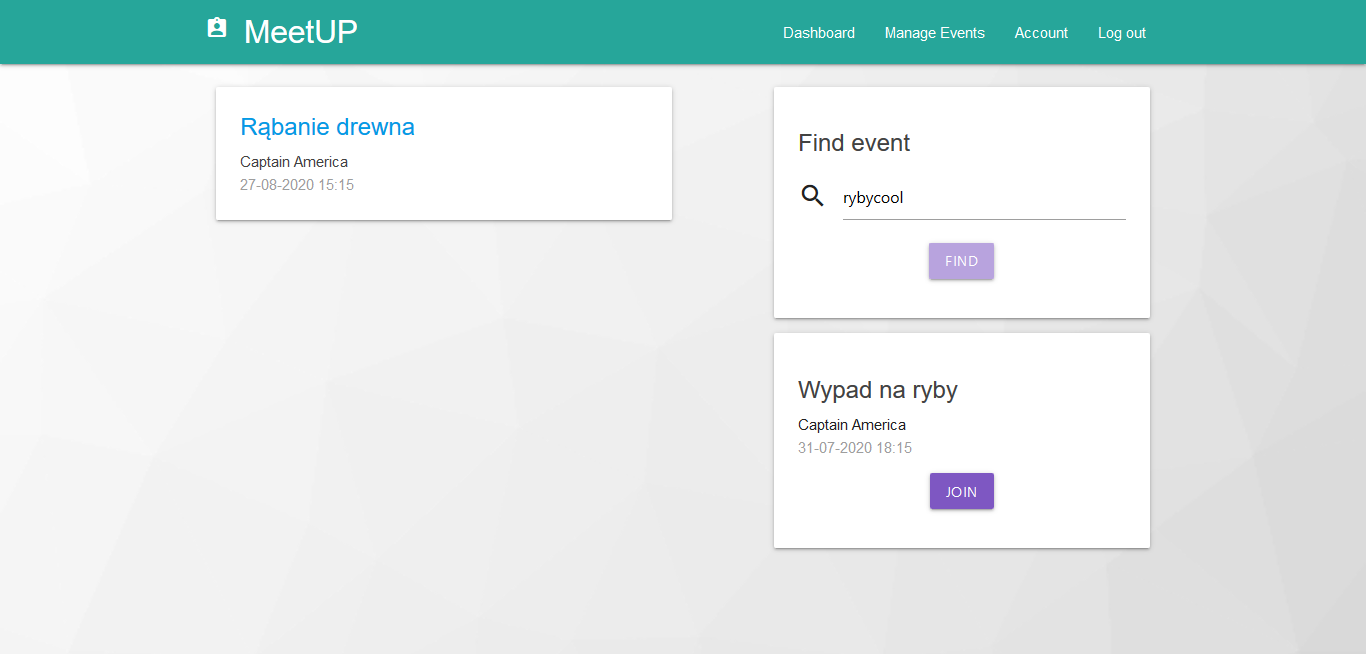
\includegraphics[width=0.9\textwidth]{meetup_find_event.png}
\caption{Wyszukiwanie wydarzenia.}
\end{figure}

Gdy wydarzenie zostanie odnalezione (w razie niepowodzenia użytkownik zostanie poinformowany), można do niego dołączyć za pomocą przycisku $JOIN$. Po tej czynności wydarzenie zostanie dodane na listę wydarzeń użytkownika.

Poprzez kliknięcie na nazwę wydarzenia na stronie głównej można przeglądać jego szczegóły. Przykładowy widok znajduje się poniżej.

\begin{figure}[H]
\centering
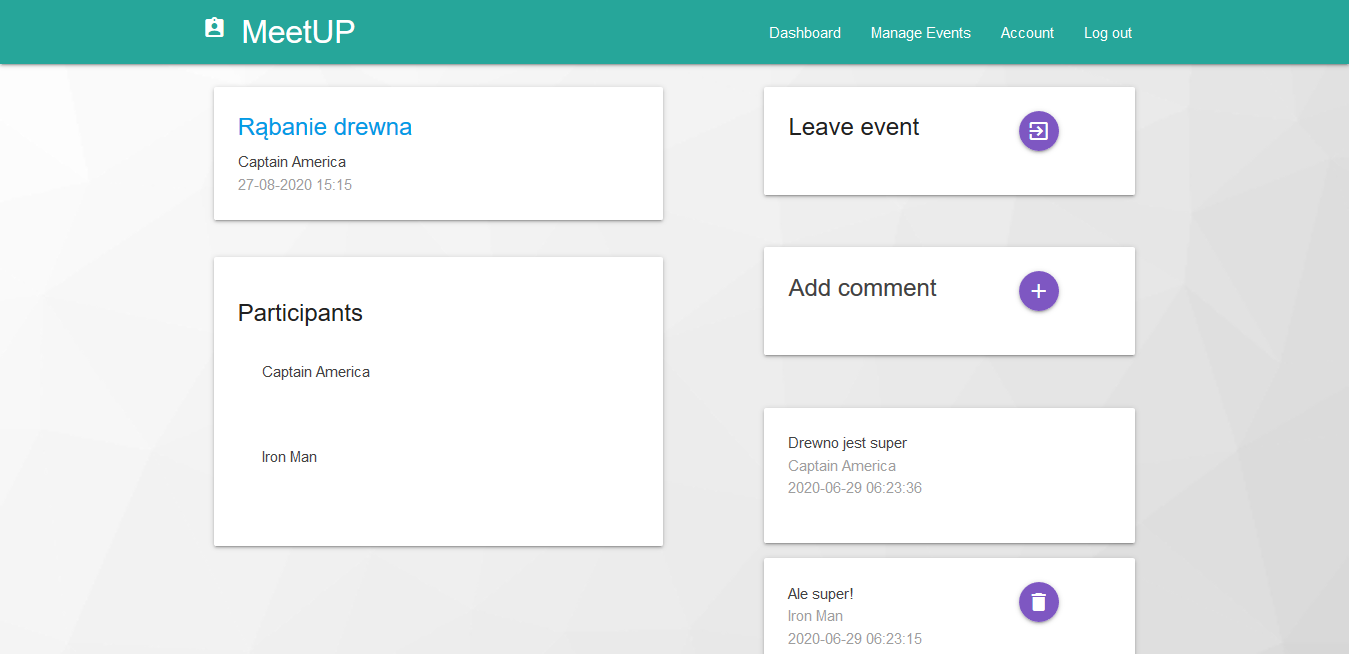
\includegraphics[width=0.9\textwidth]{meetup_event_details.png}
\caption{Szczegóły wydarzenia.}
\end{figure}

Na karcie po lewej stronie można znaleźć nazwę, organizatora oraz datę wydarzenia. Poniżej znajduje się lista wszystkich uczestników.

Po prawej stronie znajduje się panel do opuszczenia wydarzenia, do dodania komentarza oraz chronologiczna lista komentarzy. Organizator nie może opuścić wydarzenia - jedynie je usunąć. Użytkownik ma możliwość usunięcia komentarzy, których jest autorem.

\subsection{Tworzenie nowych wydarzeń}

W zakładce \textit{Manage events} użytkownik ma możliwość zarządzania wydarzeniami, których jest autorem.

\begin{figure}[H]
\centering
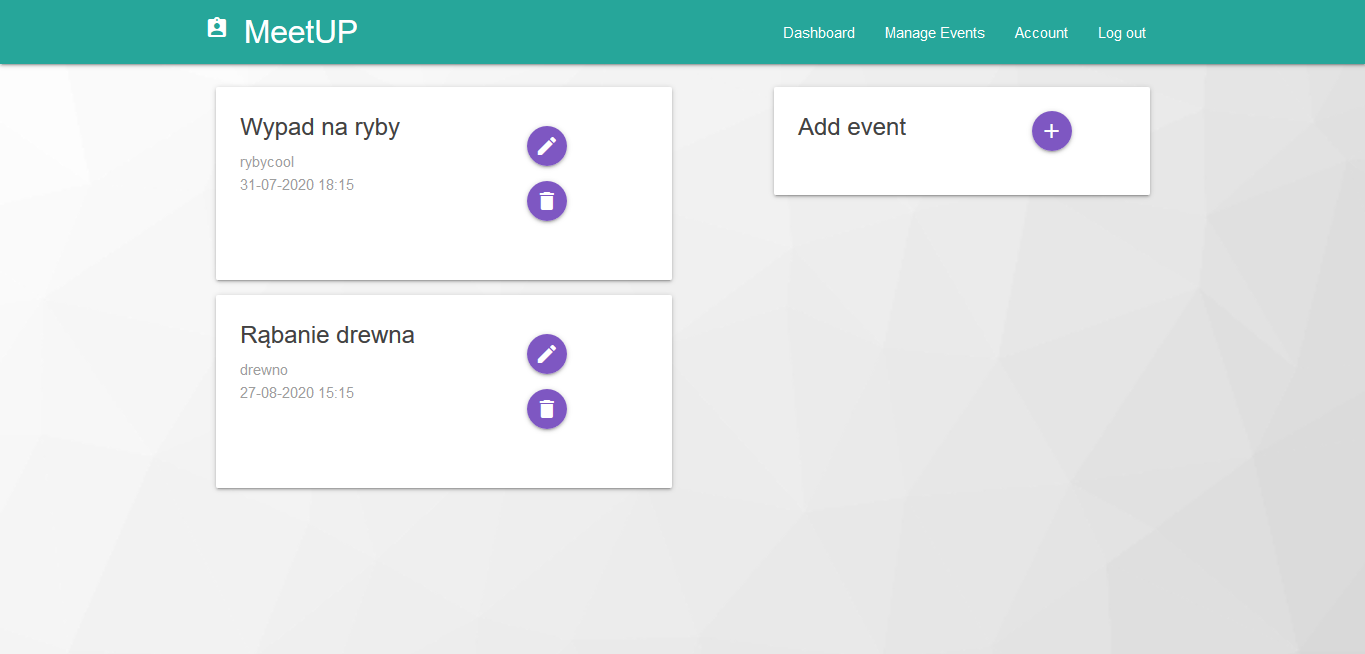
\includegraphics[width=0.9\textwidth]{meetup_manage.png}
\caption{Zarządzanie wydarzeniami.}
\end{figure}

Strona ta wygląda podobnie jak \textit{Dashboard}, ale w tym przypadku użytkownik może edytować lub usunąć wydarzenia oraz dodać nowe. Przykładowe widoki zostały przedstawione poniżej.

\begin{figure}[H]
\centering
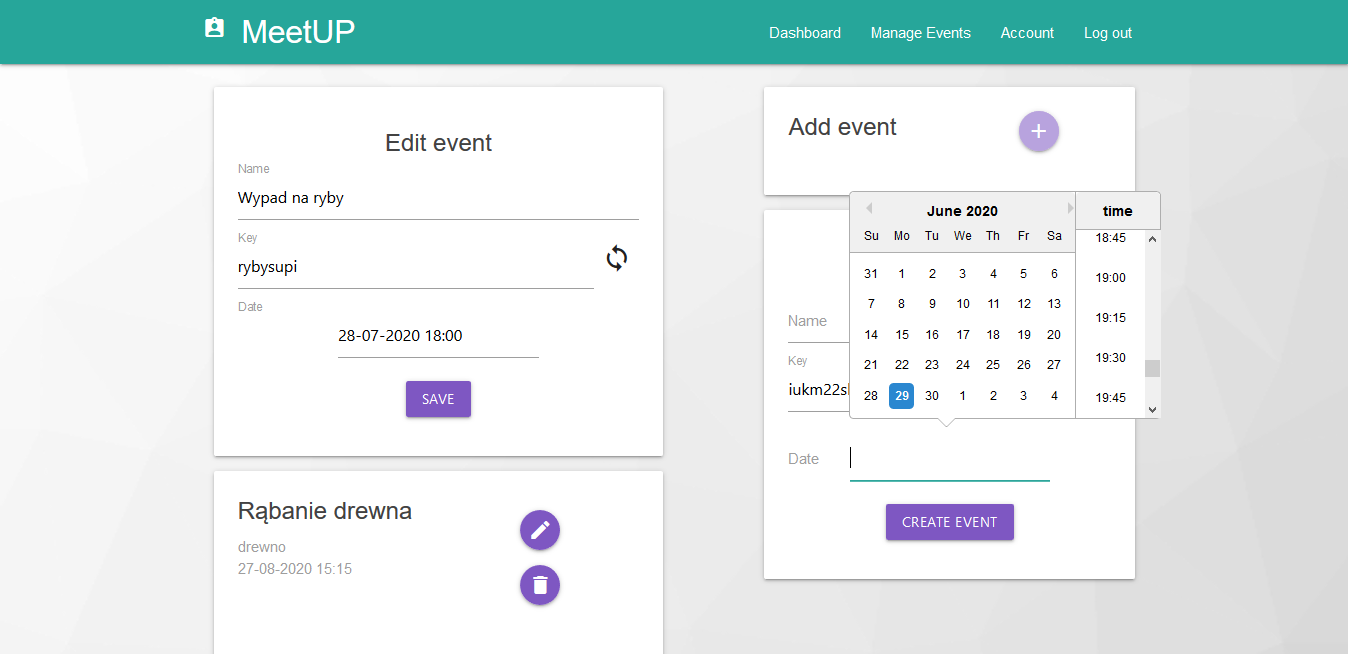
\includegraphics[width=0.9\textwidth]{meetup_manage_form.png}
\caption{Zarządzanie wydarzeniami - formularze.}
\end{figure}

Dodając bądź edytując wydarzenie użytkownik może wybrać datę z wygodnego widgetu i skorzystać z losowego generatora kluczy, bądź ustawić własny. Po zatwierdzeniu operacji przyciskiem dane zostają zapisane.

\end{document}